%!TEX TS-program = xelatex
%!TEX encoding = UTF-8 Unicode

\documentclass[School=Harvard]{Dissertate}

\geometry{letterpaper, margin=1in}

\usepackage{pdfpages}

\usepackage{color}
\definecolor{bluekeywords}{rgb}{0.13,0.13,1}
\definecolor{greencomments}{rgb}{0,0.5,0}
\definecolor{redstrings}{rgb}{0.9,0,0}
\definecolor{grey}{rgb}{0.5,0.5,0.5}

\usepackage{listings}
\lstset{
    basicstyle=\scriptsize\ttfamily,
    breakatwhitespace=false,
    breaklines=false,
    commentstyle=\color{greencomments},
    escapeinside={(*@}{@*)},
    keywordstyle=\color{bluekeywords}\bfseries,
    language=Python,
    numbers=left,
    numbersep=5pt,
    numberstyle=\tiny\color{grey},
    showspaces=false,
    showstringspaces=false,
    showtabs=false,
    stringstyle=\color{redstrings}
}

%\includeonly{source/chapters/time}

\begin{document}

\frontmatter
\pagenumbering{roman}
% Some details about the dissertation.
\title{How to cook an egg}
\author{Josiah Wolf Oberholtzer}
\advisor{Hans Tutschku \& Chaya Czernowin}

% ... about the degree.
\degree{Doctor of Philosophy}
\field{Music Composition}
\degreeyear{2015}
\degreemonth{May}
\department{Music}

% ... about the candidate's previous degrees.
\pdOneName{B.Mus.}
\pdOneSchool{Oberlin Conservatory}
\pdOneYear{2006}

%\pdTwoName{M.A.}
%\pdTwoSchool{Monster's Univeristy}
%\pdTwoYear{2021}
\maketitle
\copyrightpage
\abstractpage
\tableofcontents
%\listoffigures
\dedicationpage
\acknowledgments

\mainmatter
\doublespacing
\cleardoublepage
\pagenumbering{arabic}
\setcounter{page}{1}
\setcounter{chapter}{-1}

%%%%%%%%%%%%%%%%%%%%%%%%%%%%%%%%%%%%%%%%%%%%%%%%%%%%%%%%%%%%%%%%%%%%%%%%%%%%%%%
%%%%%%%%%%%%%%%%%%%%%%%%%%%%%%%%%%%%%%%%%%%%%%%%%%%%%%%%%%%%%%%%%%%%%%%%%%%%%%%
\chapter{Introduction}
\label{chap:introduction}
%%%%%%%%%%%%%%%%%%%%%%%%%%%%%%%%%%%%%%%%%%%%%%%%%%%%%%%%%%%%%%%%%%%%%%%%%%%%%%%
%%%%%%%%%%%%%%%%%%%%%%%%%%%%%%%%%%%%%%%%%%%%%%%%%%%%%%%%%%%%%%%%%%%%%%%%%%%%%%%

Foo

%%%%%%%%%%%%%%%%%%%%%%%%%%%%%%%%%%%%%%%%%%%%%%%%%%%%%%%%%%%%%%%%%%%%%%%%%%%%%%%
\section{Formalized score control?}
%%%%%%%%%%%%%%%%%%%%%%%%%%%%%%%%%%%%%%%%%%%%%%%%%%%%%%%%%%%%%%%%%%%%%%%%%%%%%%%

Foo

%%%%%%%%%%%%%%%%%%%%%%%%%%%%%%%%%%%%%%%%%%%%%%%%%%%%%%%%%%%%%%%%%%%%%%%%%%%%%%%
\section{Personal Background}
%%%%%%%%%%%%%%%%%%%%%%%%%%%%%%%%%%%%%%%%%%%%%%%%%%%%%%%%%%%%%%%%%%%%%%%%%%%%%%%

Foo

%%%%%%%%%%%%%%%%%%%%%%%%%%%%%%%%%%%%%%%%%%%%%%%%%%%%%%%%%%%%%%%%%%%%%%%%%%%%%%%
\section{Historical Background}
%%%%%%%%%%%%%%%%%%%%%%%%%%%%%%%%%%%%%%%%%%%%%%%%%%%%%%%%%%%%%%%%%%%%%%%%%%%%%%%

Foo

%%%%%%%%%%%%%%%%%%%%%%%%%%%%%%%%%%%%%%%%%%%%%%%%%%%%%%%%%%%%%%%%%%%%%%%%%%%%%%%
\section{\emph{Mise-en-place}: composing at the command-line}
%%%%%%%%%%%%%%%%%%%%%%%%%%%%%%%%%%%%%%%%%%%%%%%%%%%%%%%%%%%%%%%%%%%%%%%%%%%%%%%

foo

\subsection{Python}

\begin{singlespacing}
\vspace{-0.5\baselineskip}
\begin{lstlisting}
workstation:~ josiah\$ python
Python 2.7.8 (v2.7.8:ee879c0ffa11, Jun 29 2014, 21:07:35)
[GCC 4.2.1 (Apple Inc. build 5666) (dot 3)] on darwin
Type "help", "copyright", "credits" or "license" for more information.
>>>
\end{lstlisting}
\end{singlespacing}

\begin{comment}
<abjad>
1 + 1
</abjad>
\end{comment}

%%% ABJADBOOK START %%%
\begin{singlespacing}
\vspace{-0.5\baselineskip}
\begin{lstlisting}
>>> 1 + 1
2
\end{lstlisting}
\end{singlespacing}
%%% ABJADBOOK END %%%

\subsection{LilyPond}

foo

\begin{singlespacing}
\vspace{-0.5\baselineskip}
\begin{multicols}{2}
\lstinputlisting[language=]{assets/example-es-ist-genug.ly}
\vfill
\columnbreak
\setlength\fboxsep{0pt}
\setlength\fboxrule{0.5pt}
\noindent\fbox{
    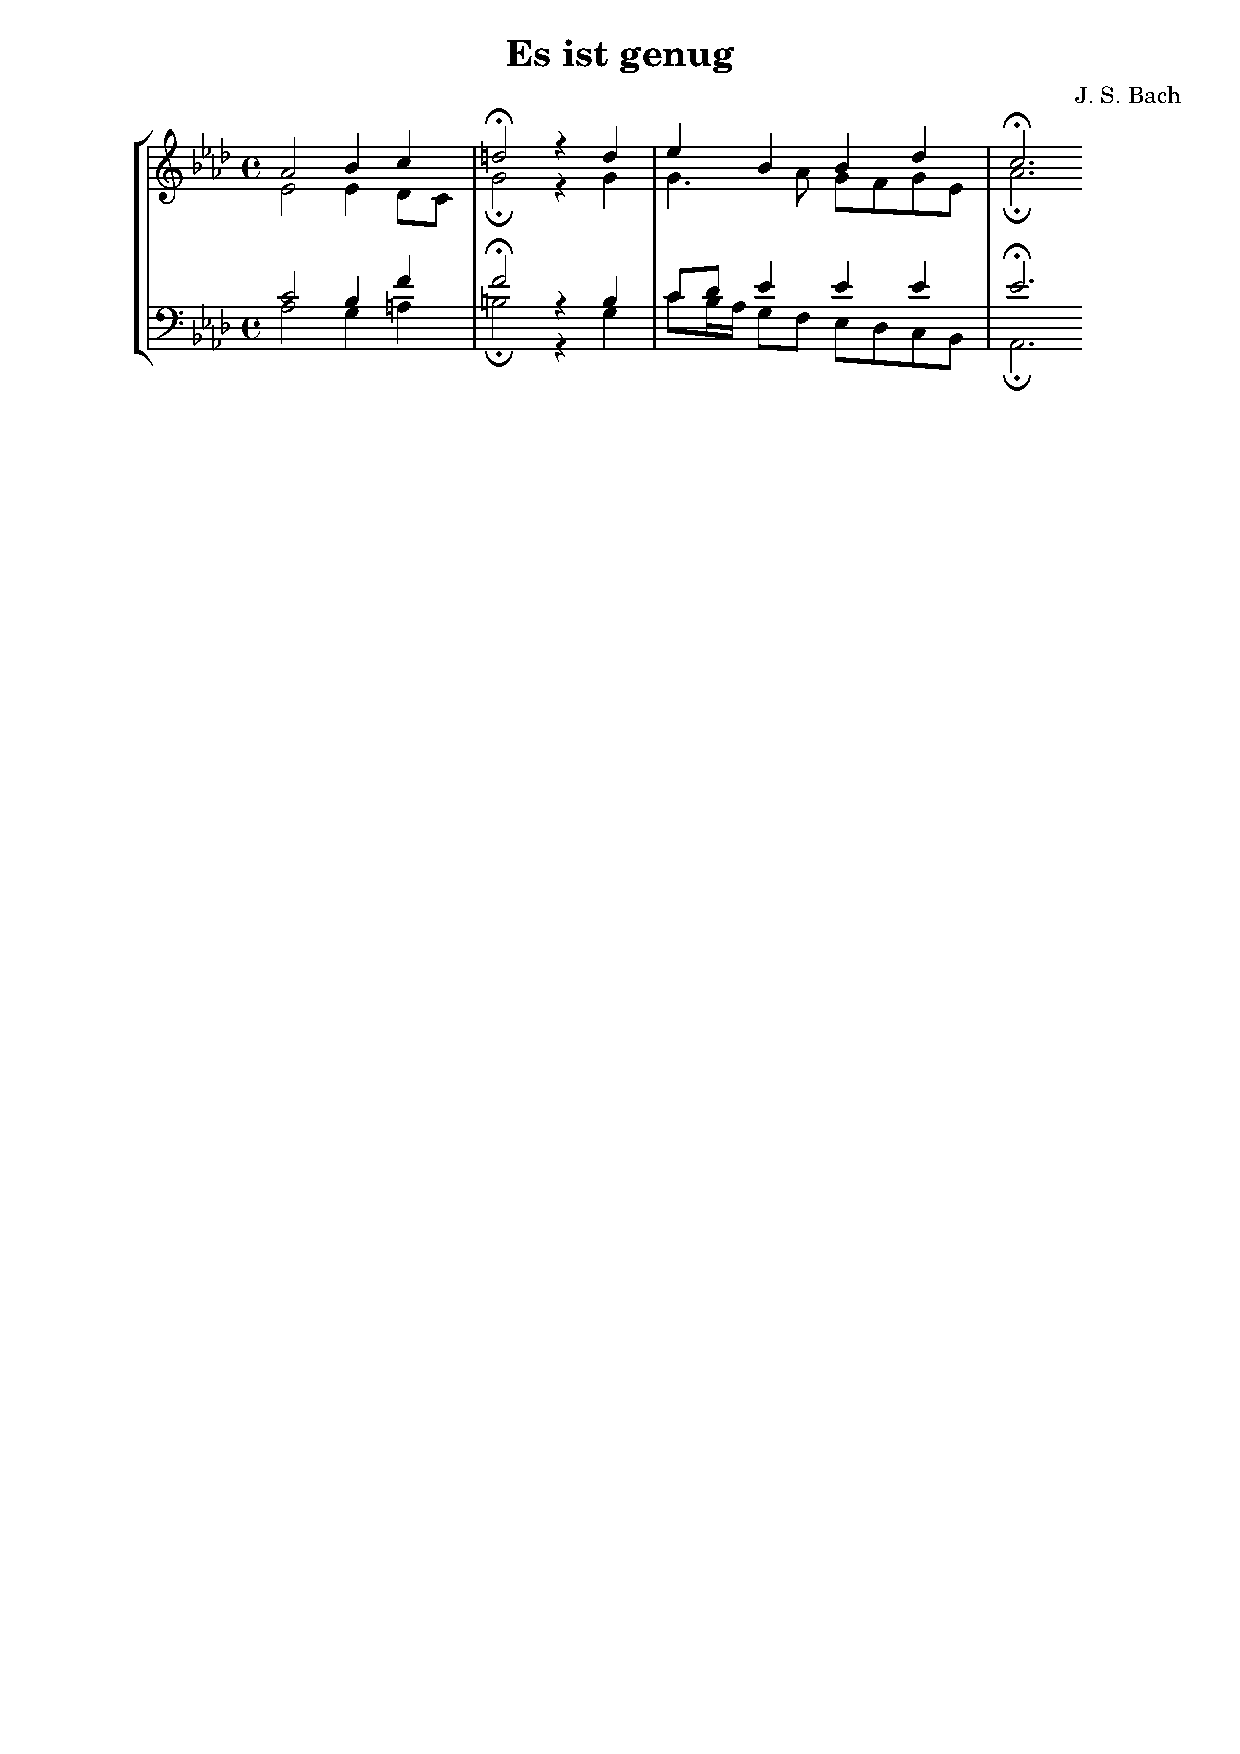
\includegraphics[scale=0.3875]{assets/example-es-ist-genug.pdf}
}
\end{multicols}
\end{singlespacing}

foo

\subsection{LaTeX}

foo

\begin{singlespacing}
\vspace{-0.5\baselineskip}
\begin{multicols}{2}
\lstinputlisting[style=beep]{assets/example-document.tex}
\vfill
\columnbreak
\setlength\fboxsep{0pt}
\setlength\fboxrule{0.5pt}
\noindent\fbox{
    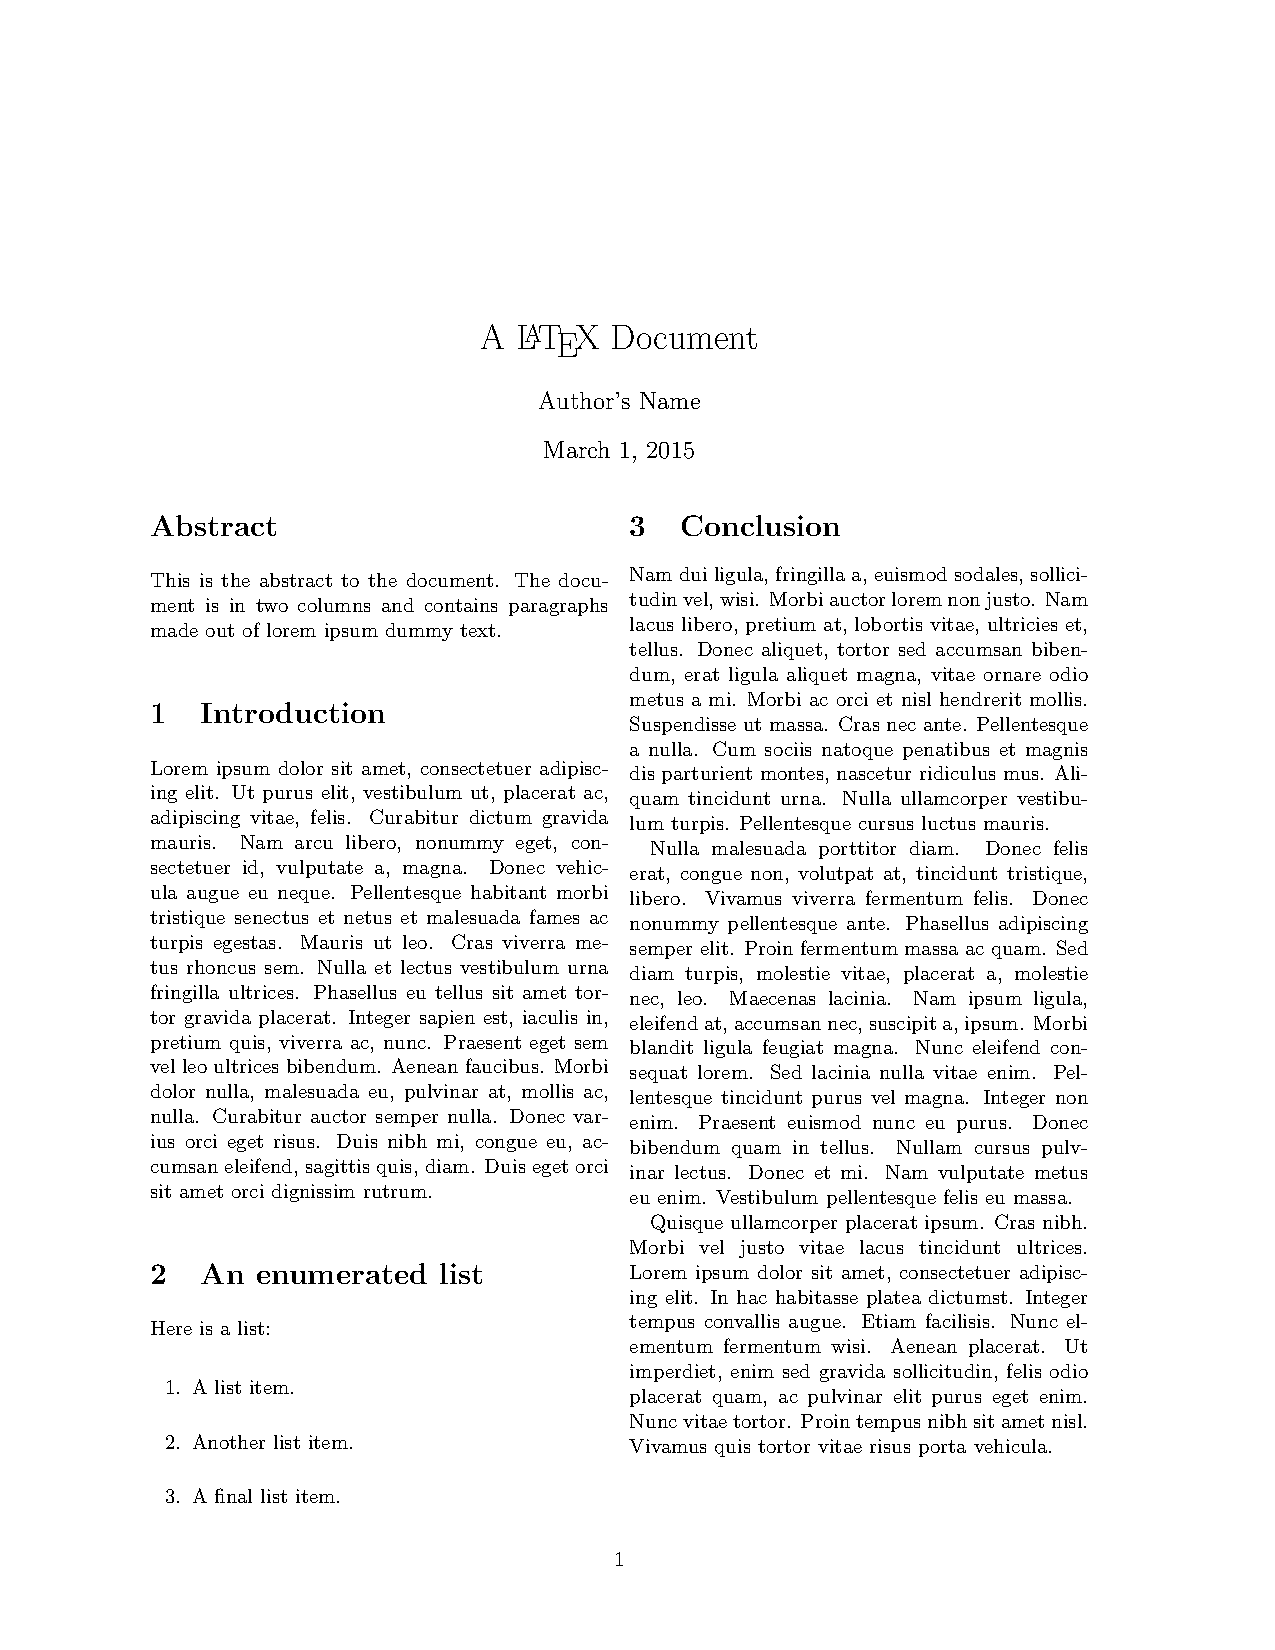
\includegraphics[scale=0.3875]{assets/example-document.pdf}
}
\end{multicols}
\end{singlespacing}

\subsection{Abjad}

foo

\subsection{Consort}

foo

%%%%%%%%%%%%%%%%%%%%%%%%%%%%%%%%%%%%%%%%%%%%%%%%%%%%%%%%%%%%%%%%%%%%%%%%%%%%%%%
\section{Motivation}
%%%%%%%%%%%%%%%%%%%%%%%%%%%%%%%%%%%%%%%%%%%%%%%%%%%%%%%%%%%%%%%%%%%%%%%%%%%%%%%

foo

%%%%%%%%%%%%%%%%%%%%%%%%%%%%%%%%%%%%%%%%%%%%%%%%%%%%%%%%%%%%%%%%%%%%%%%%%%%%%%%
\chapter{\emph{Mise-en-place}}
%%%%%%%%%%%%%%%%%%%%%%%%%%%%%%%%%%%%%%%%%%%%%%%%%%%%%%%%%%%%%%%%%%%%%%%%%%%%%%%

foo

%%%%%%%%%%%%%%%%%%%%%%%%%%%%%%%%%%%%%%%%%%%%%%%%%%%%%%%%%%%%%%%%%%%%%%%%%%%%%%%
\section{Composing at the command-line}
%%%%%%%%%%%%%%%%%%%%%%%%%%%%%%%%%%%%%%%%%%%%%%%%%%%%%%%%%%%%%%%%%%%%%%%%%%%%%%%

foo

%%%%%%%%%%%%%%%%%%%%%%%%%%%%%%%%%%%%%%%%%%%%%%%%%%%%%%%%%%%%%%%%%%%%%%%%%%%%%%%
\section{LaTeX}
%%%%%%%%%%%%%%%%%%%%%%%%%%%%%%%%%%%%%%%%%%%%%%%%%%%%%%%%%%%%%%%%%%%%%%%%%%%%%%%

foo

%%%%%%%%%%%%%%%%%%%%%%%%%%%%%%%%%%%%%%%%%%%%%%%%%%%%%%%%%%%%%%%%%%%%%%%%%%%%%%%
\section{LilyPond}
%%%%%%%%%%%%%%%%%%%%%%%%%%%%%%%%%%%%%%%%%%%%%%%%%%%%%%%%%%%%%%%%%%%%%%%%%%%%%%%

foo

%%%%%%%%%%%%%%%%%%%%%%%%%%%%%%%%%%%%%%%%%%%%%%%%%%%%%%%%%%%%%%%%%%%%%%%%%%%%%%%
\section{Python}
%%%%%%%%%%%%%%%%%%%%%%%%%%%%%%%%%%%%%%%%%%%%%%%%%%%%%%%%%%%%%%%%%%%%%%%%%%%%%%%

foo

%%%%%%%%%%%%%%%%%%%%%%%%%%%%%%%%%%%%%%%%%%%%%%%%%%%%%%%%%%%%%%%%%%%%%%%%%%%%%%%
\section{Abjad}
%%%%%%%%%%%%%%%%%%%%%%%%%%%%%%%%%%%%%%%%%%%%%%%%%%%%%%%%%%%%%%%%%%%%%%%%%%%%%%%

foo

%%%%%%%%%%%%%%%%%%%%%%%%%%%%%%%%%%%%%%%%%%%%%%%%%%%%%%%%%%%%%%%%%%%%%%%%%%%%%%%
\section{Consort}
%%%%%%%%%%%%%%%%%%%%%%%%%%%%%%%%%%%%%%%%%%%%%%%%%%%%%%%%%%%%%%%%%%%%%%%%%%%%%%%

foo

%%%%%%%%%%%%%%%%%%%%%%%%%%%%%%%%%%%%%%%%%%%%%%%%%%%%%%%%%%%%%%%%%%%%%%%%%%%%%%%
\section{Git and Vim}
%%%%%%%%%%%%%%%%%%%%%%%%%%%%%%%%%%%%%%%%%%%%%%%%%%%%%%%%%%%%%%%%%%%%%%%%%%%%%%%

foo
\chapter{\emph{Abjad}: a musical model}

foo

\section{Score components: leaves \& containers}

foo

\section{Durations, offsets and timespans}

foo

\section{Indicators: context scope and annotations}

foo

\section{Spanners}

foo

\section{Score traversal}

foo

\section{Selections and selectors}

foo

\section{Output: LilyPond format bundles}

foo

\section{Agents}

foo
\chapter{\emph{Consort}: A theory of composition}

foo
\chapter{Modeling time, rhythm and meter}

\begin{comment}
<abjad>[hide=true]
import consort
</abjad>
\end{comment}

Consort's implementation of a model of composition relies on a number of
different but interrelated models of musical time.

Dichotomies: outside and inside the score hierarchy, with or without regard to
notation, "coarse" versus "fine" or "phrase" versus "event", vertical or
horizontal, metered and unmetered, potentially simultaneous or strictly
contiguous.

Timespans provide a coarse model of musical time, both in and outside of score
hierarchy.

Notated rhythm provides a fine model of musical time, from within score
hierarchy.

Meter coordinates time and rhythm vertically across score hierarchy, and
bridges the coarse and fine stages of rhythmic interpretation.

Meter is generated as a by-product of phrase-level composition. It is not
specified by-hand during composition. This is not out of any desire to valorize
automaticism, but simply because lacking any other compelling reason to
generate a series of meters I felt the best way for myself would be to have
those meters derive from some sort of pre-existent structure in my
compositional process.

A discussion of these time models and their implications will clarify a later
analysis of the implementation of Consort's score interpretation
stage.

\section{timespans and timespan inventories}

\subsection{anatomy of a timespan}

\begin{comment}
<abjad>
timespan = timespantools.Timespan(
    start_offset=Offset(1, 4),
    stop_offset=Offset(3, 2),
    )
</abjad>
\end{comment}

\begin{comment}
<abjad>
timespan.start_offset
</abjad>
\end{comment}

\begin{comment}
<abjad>
timespan.stop_offset
</abjad>
\end{comment}

\begin{comment}
<abjad>
timespan.duration
</abjad>
\end{comment}

\begin{comment}
<abjad>
timespan.is_well_formed
</abjad>
\end{comment}

\begin{comment}
<abjad>
malformed_timespan = timespantools.Timespan(0, 0)
malformed_timespan.is_well_formed
</abjad>
\end{comment}

\begin{comment}
<abjad>
templated_timespan = new(timespan, stop_offset=(5, 16))
print(format(templated_timespan))
</abjad>
\end{comment}

\begin{comment}
<abjad>
annotated_timespan = timespantools.AnnotatedTimespan(
    start_offset=(1, 8),
    stop_offset=(7, 8),
    annotation='Any arbitrary object can act as an annotation.'
    )
annotated_timespan.annotation
</abjad>
\end{comment}

\subsection{time relations}

- comparison

- time relations: intersection, congruency etc.

\begin{comment}
<abjad>
timespan_1 = timespantools.Timespan(0, 10)
timespan_2 = timespantools.Timespan(5, 15)
timespan_3 = timespantools.Timespan(10, 15)
</abjad>
\end{comment}

\begin{comment}
<abjad>
timespan_1.intersects_timespan(timespan_2)
timespan_1.intersects_timespan(timespan_3)
timespan_2.intersects_timespan(timespan_1)
timespan_2.intersects_timespan(timespan_3)
timespan_3.intersects_timespan(timespan_1)
timespan_3.intersects_timespan(timespan_2)
</abjad>
\end{comment}

\begin{comment}
<abjad>
timespan_1.is_congruent_to_timespan(timespan_2)
timespan_1.is_congruent_to_timespan(timespan_1)
</abjad>
\end{comment}

\begin{comment}
<abjad>
timespan_1.is_tangent_to_timespan(timespan_2)
timespan_1.is_tangent_to_timespan(timespan_3)
</abjad>
\end{comment}

- operations

Consider the following three timespans again.

\begin{comment}
<abjad>
timespan_1 = timespantools.Timespan(0, 10)
timespan_2 = timespantools.Timespan(5, 15)
timespan_3 = timespantools.Timespan(10, 15)
</abjad>
\end{comment}

The logical AND of any two timespans can be computed.

\begin{comment}
<abjad>
timespan_1 & timespan_2
timespan_1 & timespan_3
timespan_2 & timespan_3
</abjad>
\end{comment}

The logical OR of any two timespans can be computed.

\begin{comment}
<abjad>
timespan_1 | timespan_2
timespan_1 | timespan_3
timespan_2 | timespan_3
</abjad>
\end{comment}

Timespan subtraction is another crucial operation.

\begin{comment}
<abjad>
timespan_1 = timespantools.Timespan(0, 15)
timespan_2 = timespantools.Timespan(5, 10)
timespan_3 = timespantools.Timespan(10, 20)
</abjad>
\end{comment}

\begin{comment}
<abjad>
print(format(timespan_1 - timespan_1))
print(format(timespan_1 - timespan_2))
print(format(timespan_1 - timespan_3))
print(format(timespan_2 - timespan_1))
print(format(timespan_2 - timespan_2))
print(format(timespan_2 - timespan_3))
print(format(timespan_3 - timespan_1))
print(format(timespan_3 - timespan_2))
print(format(timespan_3 - timespan_3))
</abjad>
\end{comment}

\subsection{aggregate operations}

Timespans can be aggregated together in an instance of the TimespanInventory
class. In addition to the protocol defined for ordered collections, timespan
inventories provide a variety of other methods and properties for working
specifically with timespans.

\begin{comment}
<abjad>
timespan_inventory = timespantools.TimespanInventory([
    timespantools.Timespan(0, 16),
    timespantools.Timespan(5, 12),
    timespantools.Timespan(-2, 8),
    ])
timespan_inventory.timespan
timespan_inventory.duration
timespan_inventory.start_offset
timespan_inventory.stop_offset
timespan_inventory.append(timespantools.Timespan(15, 20))
timespan_inventory.sort()
timespan_inventory.duration
</abjad>
\end{comment}

- unioning, differencing and splitting

\begin{comment}
<abjad>
timespan_inventory = timespantools.TimespanInventory([
    timespantools.Timespan(0, 16),
    timespantools.Timespan(5, 12),
    timespantools.Timespan(-2, 8),
    ])
timespan = timespantools.Timespan(5, 10)
result = timespan_inventory & timespan
print(format(timespan_inventory))
</abjad>
\end{comment}

\begin{comment}
<abjad>
timespan_inventory = timespantools.TimespanInventory([
    timespantools.Timespan(0, 16),
    timespantools.Timespan(5, 12),
    timespantools.Timespan(-2, 8),
    ])
timespan = timespantools.Timespan(5, 10)
result = timespan_inventory - timespan
print(format(timespan_inventory))
</abjad>
\end{comment}

\begin{comment}
<abjad>
timespan_inventory = timespantools.TimespanInventory([
    timespantools.Timespan(0, 3),
    timespantools.Timespan(3, 6),
    timespantools.Timespan(6, 10),
    ])
left, right = timespan_inventory.split_at_offset(4)
print(format(left))
print(format(right))
</abjad>
\end{comment}

Timespan.split_at_offsets()

- partitioning

\begin{comment}
<abjad>
timespan_inventory = timespantools.TimespanInventory([
    timespantools.Timespan(0, 10),
    timespantools.Timespan(5, 15),
    timespantools.Timespan(15, 20),
    timespantools.Timespan(25, 30),
    ])
</abjad>
\end{comment}

\begin{comment}
<abjad>
for inventory in timespan_inventory.partition():
    print(format(inventory))

</abjad>
\end{comment}

\begin{comment}
<abjad>
for inventory in timespan_inventory.partition(include_tangent_timespans=True):
    print(format(inventory))

</abjad>
\end{comment}

- multiplexing and demultiplexing

- resolution

- other operations

TimespanInventory.all_are_contiguous
TimespanInventory.all_are_nonoverlapping
TimespanInventory.clip_timespan_durations
TimespanInventory.count_offsets()
TimespanInventory.explode()
TimespanInventory.round_offsets()

- timespan collection vs timespan inventory

Consort provides its own timespan collection class -- the TimespanCollection.
This class stores timespans internally not as a list, but in a balanced
"interval tree" datastructure which guarantees sorting and allows for highly
optimized lookups of timespans intersecting specific offsets. This class is
used at crucial points during Consort's interpretation stage simply for
purposes of speed, and should be considered an implementation detail. With
work, its internal datastructure will eventually be merged into Abjad's
TimespanInventory.

\section{performed and silent timespans}

\begin{comment}
<abjad>
performed_timespan = consort.PerformedTimespan(
    layer=1,
    minimum_duration=Duration(1, 8),
    music_specifier=consort.MusicSpecifier(),
    start_offset=Offset(1, 4),
    stop_offset=Offset(2, 1),
    voice_name='Violin 1 LH Voice',
    )
</abjad>
\end{comment}

\begin{comment}
<abjad>
silent_timespan = consort.SilentTimespan(
    layer=2,
    start_offset=Offset(0, 1),
    stop_offset=Offset(1, 4),
    voice_name='Violin 1 LH Voice',
    )
</abjad>
\end{comment}

\subsection{payloaded timespans}

- layer

- voice name

\subsection{performed timespans}

- forbid fusing

- forbid splitting

- minimum duration

- (additionally, music specifier: minimum phrase duration)

- divisions

- music

- music specifier

\section{timespan makers}

- timespan specifier

- independent vs dependent

- target timespans

- talea

- padding

\subsection{flooded timespan maker}

\begin{comment}
<abjad>
flooded_timespan_maker = consort.FloodedTimespanMaker()
print(format(flooded_timespan_maker))
</abjad>
\end{comment}

\subsection{talea timespan maker}

\begin{comment}
<abjad>
timespan_maker = consort.TaleaTimespanMaker(
    initial_silence_talea=rhythmmakertools.Talea(
        counts=(0, 4),
        denominator=16,
        )
    )
</abjad>

- taleas: playing, silence and initial silence

- groupings

- synchronization

- repeat and reflect

\subsection{dependent timespan maker}

\begin{comment}
<abjad>
dependent_timespan_maker = consort.DependentTimespanMaker(
    include_inner_starts=True,
    include_inner_stops=False,
    voice_names=(
        'Piano Upper Voice',
        'Piano Lower Voice',
        )
    )
</abjad>
\end{comment}

\section{rhythm makers}

\subsection{a factory for rhythmic material}

- divisions

\begin{comment}
<abjad>
divisions = [(3, 8), (4, 8), (3, 16), (4, 16), (5, 8), (2, 4)]
</abjad>
\end{comment}

- rhythm maker

\subsection{configuration}

- specifiers: tie, duration spelling, beam

\subsection{examples}

- specific rhythm makers

- NoteRhythmMaker

\begin{comment}
<abjad>
note_rhythm_maker = rhythmmakertools.NoteRhythmMaker(
    )
show(note_rhythm_maker, divisions=divisions)
</abjad>
\end{comment}

- EvenDivisionsRhythmMaker

\begin{comment}
<abjad>
even_division_rhythm_maker = rhythmmakertools.EvenDivisionRhythmMaker(
    denominators=[8, 16, 4],
    )
show(even_division_rhythm_maker, divisions=divisions)
</abjad>
\end{comment}

- IncisedRhythmMaker

\begin{comment}
<abjad>
incised_rhythm_maker = rhythmmakertools.IncisedRhythmMaker(
    incise_specifier=rhythmmakertools.InciseSpecifier(
        prefix_counts=[0],
        suffix_talea=[-1],
        suffix_counts=[1],
        talea_denominator=16,
        ),
    )
show(incised_rhythm_maker, divisions=divisions)
</abjad>
\end{comment}

- TaleaRhythmMaker

\begin{comment}
<abjad>
talea_rhythm_maker = rhythmmakertools.TaleaRhythmMaker(
    talea=rhythmmakertools.Talea(
        counts=[1, 2, 3, 4],
        denominator=16,
        ),
    )
show(talea_rhythm_maker, divisions=divisions)
</abjad>
\end{comment}

\subsection{composite rhythm maker}

\begin{comment}
<abjad>
composite_rhythm_maker = consort.CompositeRhythmMaker(
    default=note_rhythm_maker,
    last=incised_rhythm_maker,
    first=even_division_rhythm_maker,
    )
</abjad>
\end{comment}

\section{meter finding and rewriting}

\subsection{describing meter}

- meters vs time signatures

- rhythm trees

\begin{comment}
<abjad>
three_four_meter = metertools.Meter((3, 4))
five_sixteen_meter = metertools.Meter((5, 16))
six_eight_meter = metertools.Meter((6, 8))
print(three_four_meter.pretty_rtm_format)
print(five_sixteen_meter.pretty_rtm_format)
print(six_eight_meter.pretty_rtm_format)
</abjad>
\end{comment}

\subsection{finding meters}

\begin{comment}
<abjad>
permitted_meters = [metertools.Meter(_) for _ in [(3, 4), (4, 4), (5, 4)]]
offsets = [(0, 4), (4, 4), (8, 4), (12, 4), (16, 4)]
for x in metertools.Meter.fit_meters_to_expr(offsets, permitted_meters):
    print(x.implied_time_signature)

</abjad>
\end{comment}

\begin{comment}
<abjad>
offsets = [(0, 4), (3, 4), (5, 4), (10, 4), (15, 4), (20, 4)]
for x in metertools.Meter.fit_meters_to_expr(offsets, permitted_meters):
    print(x.implied_time_signature)

</abjad>
\end{comment}

- metric accent kernels

- offset counters

- discard final silence

\subsection{rewriting meters}

- specific iteration techniques

- boundary depth

- dot count
\chapter{TimeManager: a method for laying out time}

foo
\chapter{Handlers: specifying pitch and attachment}

foo
%%%%%%%%%%%%%%%%%%%%%%%%%%%%%%%%%%%%%%%%%%%%%%%%%%%%%%%%%%%%%%%%%%%%%%%%%%%%%%%
%%%%%%%%%%%%%%%%%%%%%%%%%%%%%%%%%%%%%%%%%%%%%%%%%%%%%%%%%%%%%%%%%%%%%%%%%%%%%%%
\chapter{Conclusion}
\label{chap:conclusion}
%%%%%%%%%%%%%%%%%%%%%%%%%%%%%%%%%%%%%%%%%%%%%%%%%%%%%%%%%%%%%%%%%%%%%%%%%%%%%%%
%%%%%%%%%%%%%%%%%%%%%%%%%%%%%%%%%%%%%%%%%%%%%%%%%%%%%%%%%%%%%%%%%%%%%%%%%%%%%%%

\begin{markdown}

# Composing in text

- Allography
- Version control
- If the input is versioned text, not graphic, there is always a clear,
  retrievable history of the thought process behind the work

# Maquettes and unfolding processes

- Timespans allow for large scale phrasing and density structures.
- They simply model attack points and durations, making attack and overlap
  density easy to play with.
- Timespan annotations allow for maquette-like composition techniques, or
  working in a way that conceptually mirrors working with a DAW, even though
  there is no real graphic output except for notation itself.
- Annotations can act as a description of what sort of material should appear
  in what locations -- both horizontally in time and vertically in the score
  hierarchy.
- Timespans also allow for overlap, and have affordances for masking.
- This allows timespans to be created by a factories in layers, and those
  layers resolved down to a single non-overlapping layer via masking.

# Patterns and randomness

- All of the maker tools described here (and in the next chapter) emphasize
  working with patterns.
- Sufficiently complex patterns of discrete numbers (and combinations of
  patterns) are perceptually indistinguishable from randomness. It doesn't
  take much.
- Likewise, randomness -- no matter how it is arrived at, windowed, weighted
  and so forth -- is a kind of maintenance burden. How can you know that
  your compositional machinery is behaving correctly when the results are
  always different by design?
- Why the extensive use of patterns rather than anything else?
- Patterns are sufficient
- They are also testable

# Architecture and extensibility

- Only a few recipes for timespan and rhythm creation have been outlined
  here. Obviously, many more are possible, with other paradigms. The models
  described here generally rely on patterns. Other work could create
  rhythm-makers which take pitches as input, or which follow breakpoints, or
  mimic some other external structure. Likewise with timespan-makers. More
  work could be done to create stronger intentional interrelations between
  timespans.
- One of the strengths in the overall design philosophy described throughout
  this chapter is extensibility. Just because I *haven't* yet created a
  derived-from-bird-song rhythm-maker doesn't mean I can't. Such a maker
  could be created and follow the same interface as all other rhythm-makers,
  benefiting from their foundation of shared notational logics.
- More factories are possible
- Those outlined here are neither the *only* nor the *best* possible
  factories one could design
- New factories can make use of the interfaces implemented by these
  factory families (timespan- and rhythm-makers)
- New factories can also propose entirely new ways of working
  (such as...)
- Extensibility is afforded because the basic building blocks --
  timespans, timespan inventories, meter and Abjad's model of score --
  are rock solid

# Score as evaluable expression

# Expressivity

\end{markdown}

%%%%%%%%%%%%%%%%%%%%%%%%%%%%%%%%%%%%%%%%%%%%%%%%%%%%%%%%%%%%%%%%%%%%%%%%%%%%%%%
%%%%%%%%%%%%%%%%%%%%%%%%%%%%%%%%%%%%%%%%%%%%%%%%%%%%%%%%%%%%%%%%%%%%%%%%%%%%%%%
\chapter{\emph{Aurora} (2011)}
%%%%%%%%%%%%%%%%%%%%%%%%%%%%%%%%%%%%%%%%%%%%%%%%%%%%%%%%%%%%%%%%%%%%%%%%%%%%%%%
%%%%%%%%%%%%%%%%%%%%%%%%%%%%%%%%%%%%%%%%%%%%%%%%%%%%%%%%%%%%%%%%%%%%%%%%%%%%%%%

foo

\includepdf[
    pages=2-58,
    pagecommand={\thispagestyle{plain}},
    scale=0.9
]{assets/dissertation-score-aurora.pdf}
%%%%%%%%%%%%%%%%%%%%%%%%%%%%%%%%%%%%%%%%%%%%%%%%%%%%%%%%%%%%%%%%%%%%%%%%%%%%%%%
%%%%%%%%%%%%%%%%%%%%%%%%%%%%%%%%%%%%%%%%%%%%%%%%%%%%%%%%%%%%%%%%%%%%%%%%%%%%%%%
\chapter{\emph{Plague Water} (2014)}
%%%%%%%%%%%%%%%%%%%%%%%%%%%%%%%%%%%%%%%%%%%%%%%%%%%%%%%%%%%%%%%%%%%%%%%%%%%%%%%
%%%%%%%%%%%%%%%%%%%%%%%%%%%%%%%%%%%%%%%%%%%%%%%%%%%%%%%%%%%%%%%%%%%%%%%%%%%%%%%

foo

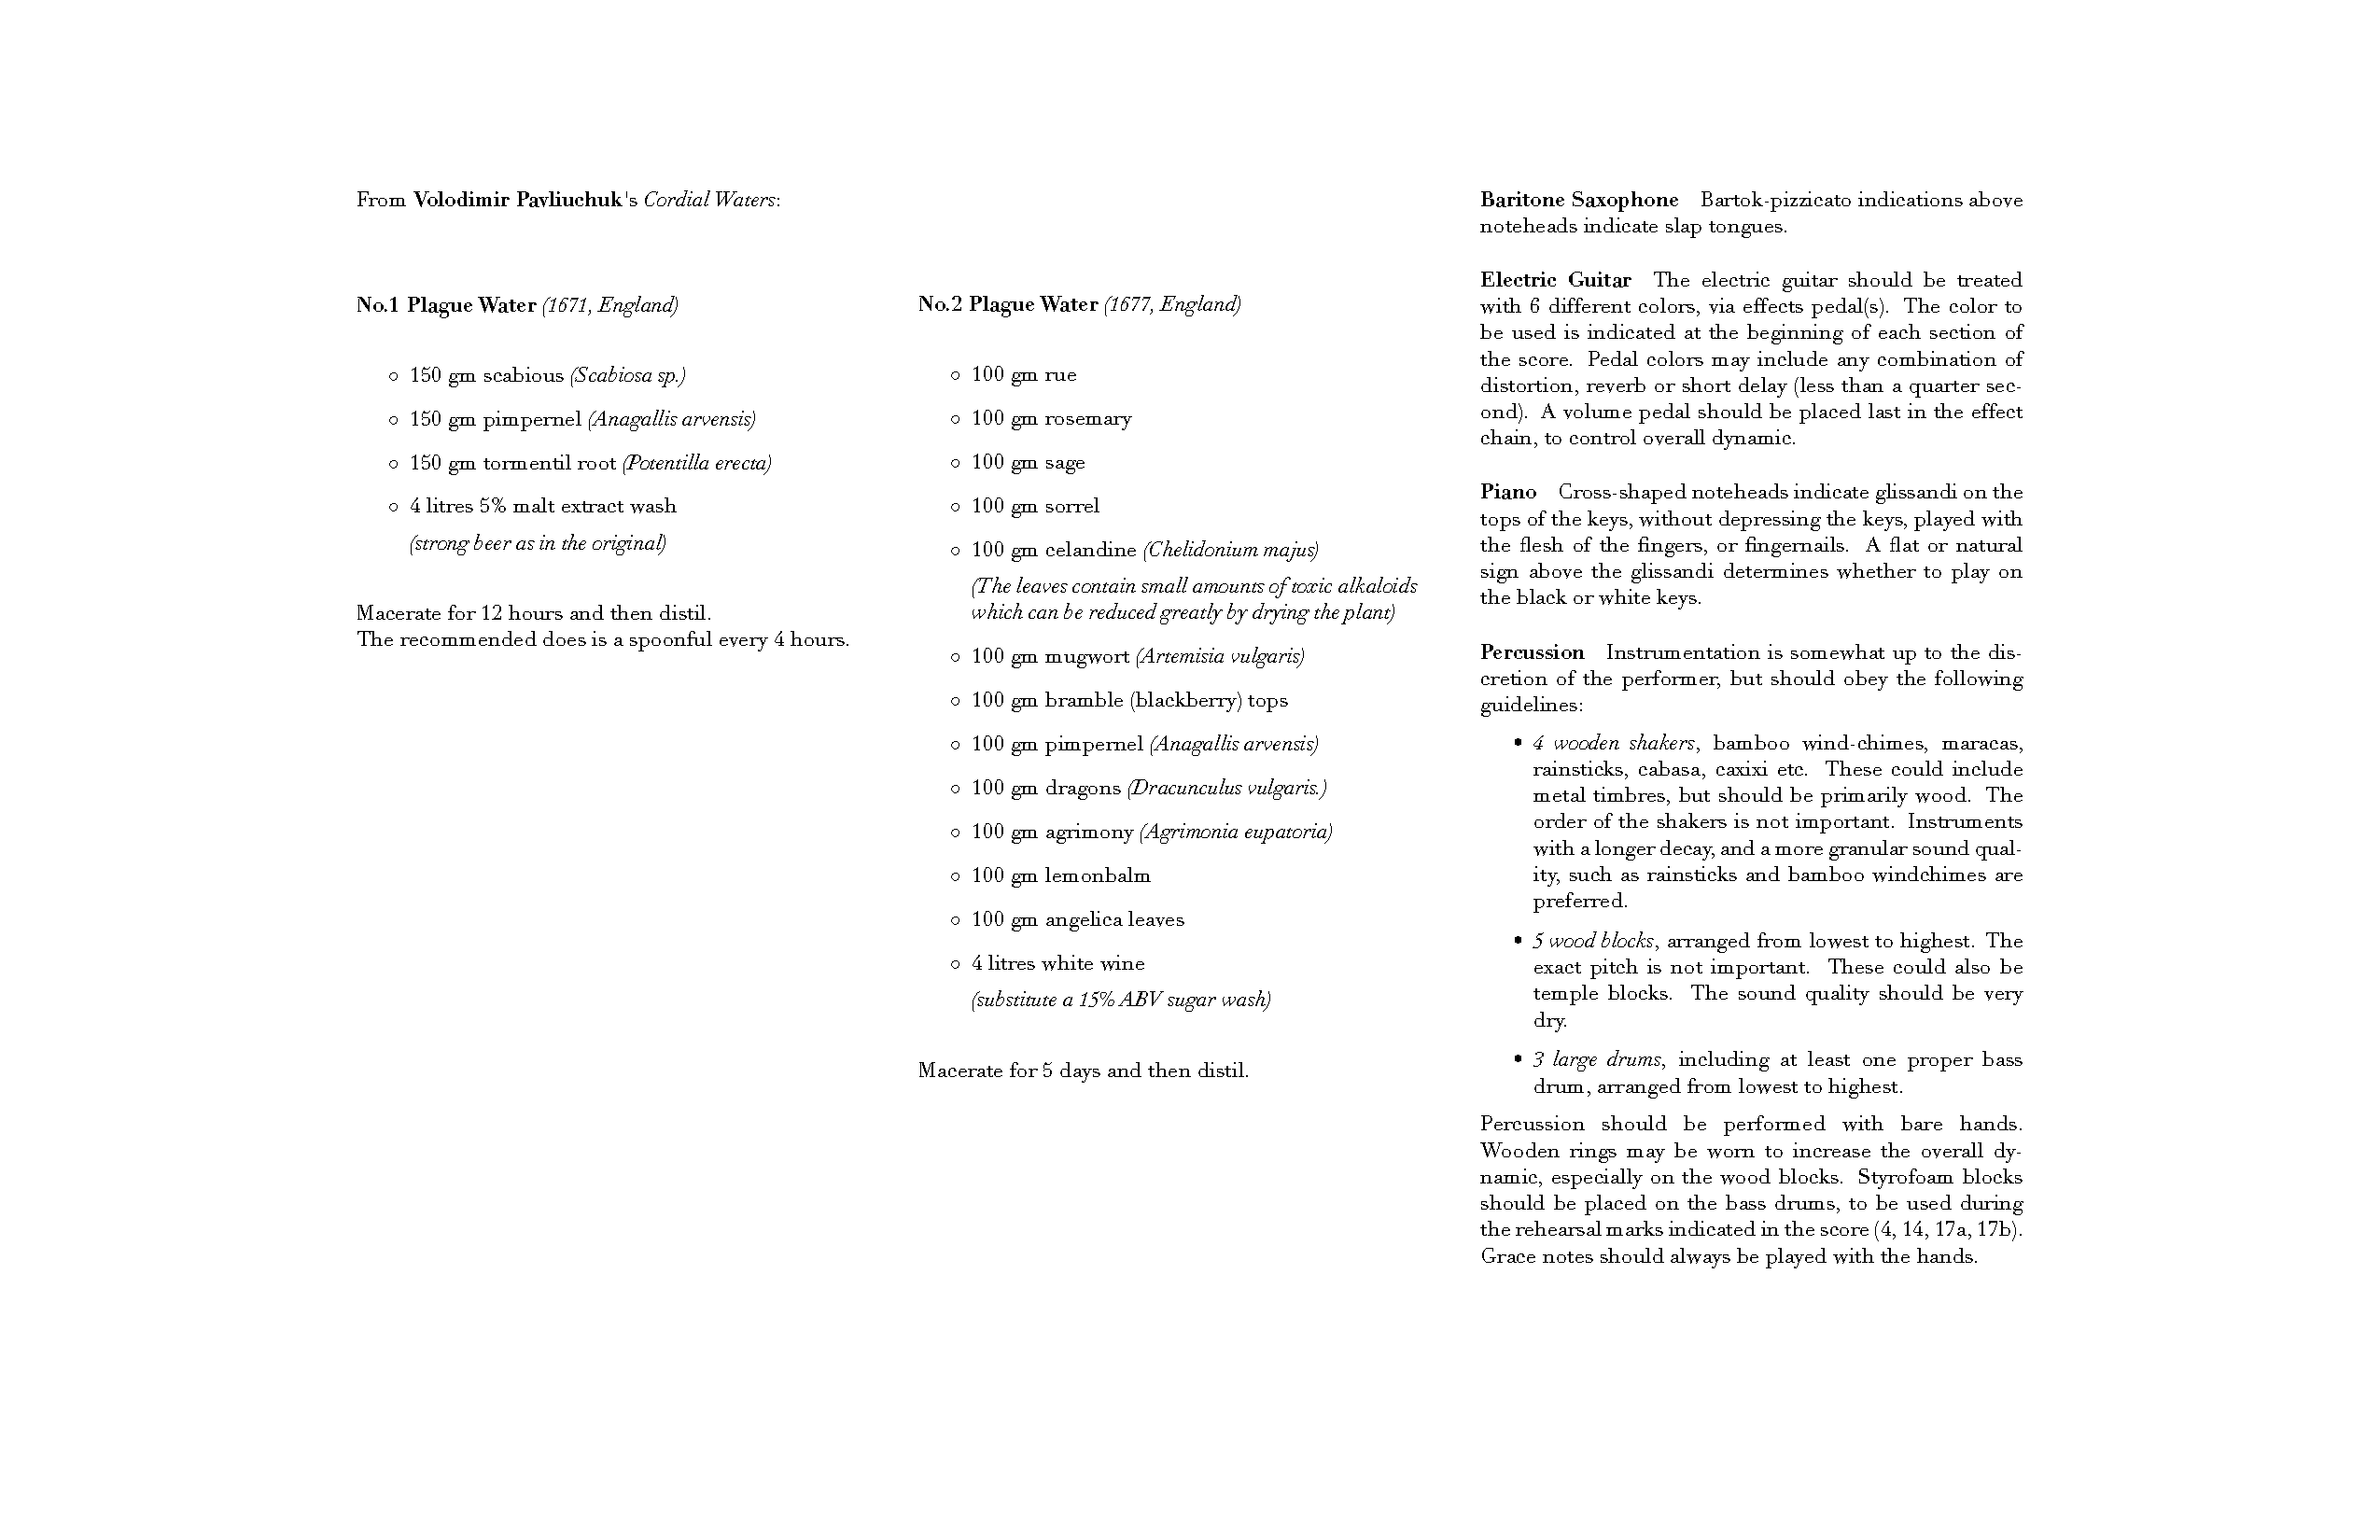
\includepdf[
    pages=-,
    pagecommand={\thispagestyle{plain}}
]{assets/dissertation-score-plague-water.pdf}
%%%%%%%%%%%%%%%%%%%%%%%%%%%%%%%%%%%%%%%%%%%%%%%%%%%%%%%%%%%%%%%%%%%%%%%%%%%%%%%
%%%%%%%%%%%%%%%%%%%%%%%%%%%%%%%%%%%%%%%%%%%%%%%%%%%%%%%%%%%%%%%%%%%%%%%%%%%%%%%
\chapter{\emph{Invisible Cities (i): Zaira} (2014)}
%%%%%%%%%%%%%%%%%%%%%%%%%%%%%%%%%%%%%%%%%%%%%%%%%%%%%%%%%%%%%%%%%%%%%%%%%%%%%%%
%%%%%%%%%%%%%%%%%%%%%%%%%%%%%%%%%%%%%%%%%%%%%%%%%%%%%%%%%%%%%%%%%%%%%%%%%%%%%%%

\begin{singlespacing}
\begin{flushright}
A composition for eight players \\
\vspace*{\baselineskip}
Premi\`{e}red by Ensemble Mosaik \\
on Saturday October 4th, 2014 \\
in Paine Hall, Harvard University
\end{flushright}
\end{singlespacing}

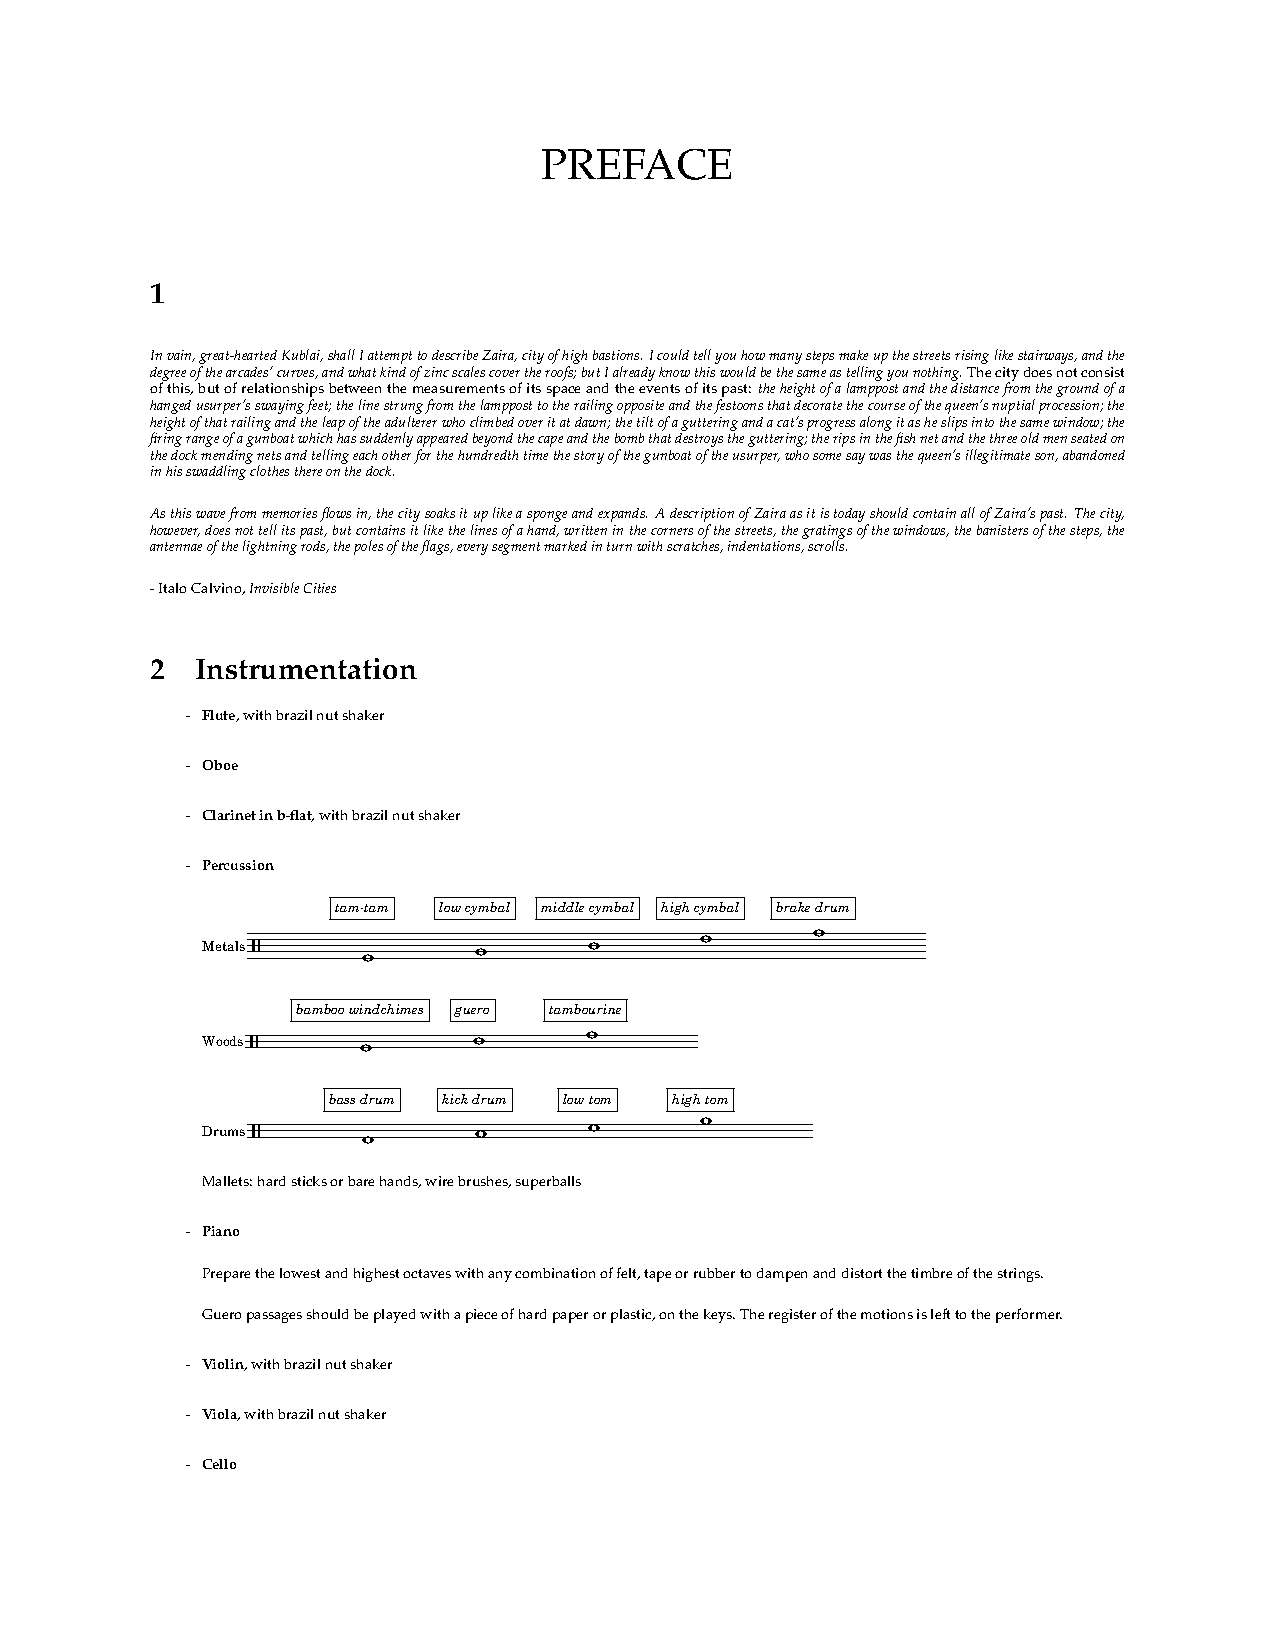
\includepdf[
    pages=-,
    pagecommand={\thispagestyle{plain}}
]{assets/dissertation-score-zaira.pdf}
%%%%%%%%%%%%%%%%%%%%%%%%%%%%%%%%%%%%%%%%%%%%%%%%%%%%%%%%%%%%%%%%%%%%%%%%%%%%%%%
%%%%%%%%%%%%%%%%%%%%%%%%%%%%%%%%%%%%%%%%%%%%%%%%%%%%%%%%%%%%%%%%%%%%%%%%%%%%%%%
\chapter{\emph{Invisible Cities (ii): Armilla} (2015)}
\label{chap:armilla}
%%%%%%%%%%%%%%%%%%%%%%%%%%%%%%%%%%%%%%%%%%%%%%%%%%%%%%%%%%%%%%%%%%%%%%%%%%%%%%%
%%%%%%%%%%%%%%%%%%%%%%%%%%%%%%%%%%%%%%%%%%%%%%%%%%%%%%%%%%%%%%%%%%%%%%%%%%%%%%%

\begin{singlespacing}
\begin{flushright}
A composition for viola duet \\
\vspace*{\baselineskip}
Premi\`{e}red by Elizabeth Weisser \& \\
John Pickford Richards \\
on Saturday February 7th, 2015 \\
in Paine Hall, Harvard University
\end{flushright}
\end{singlespacing}

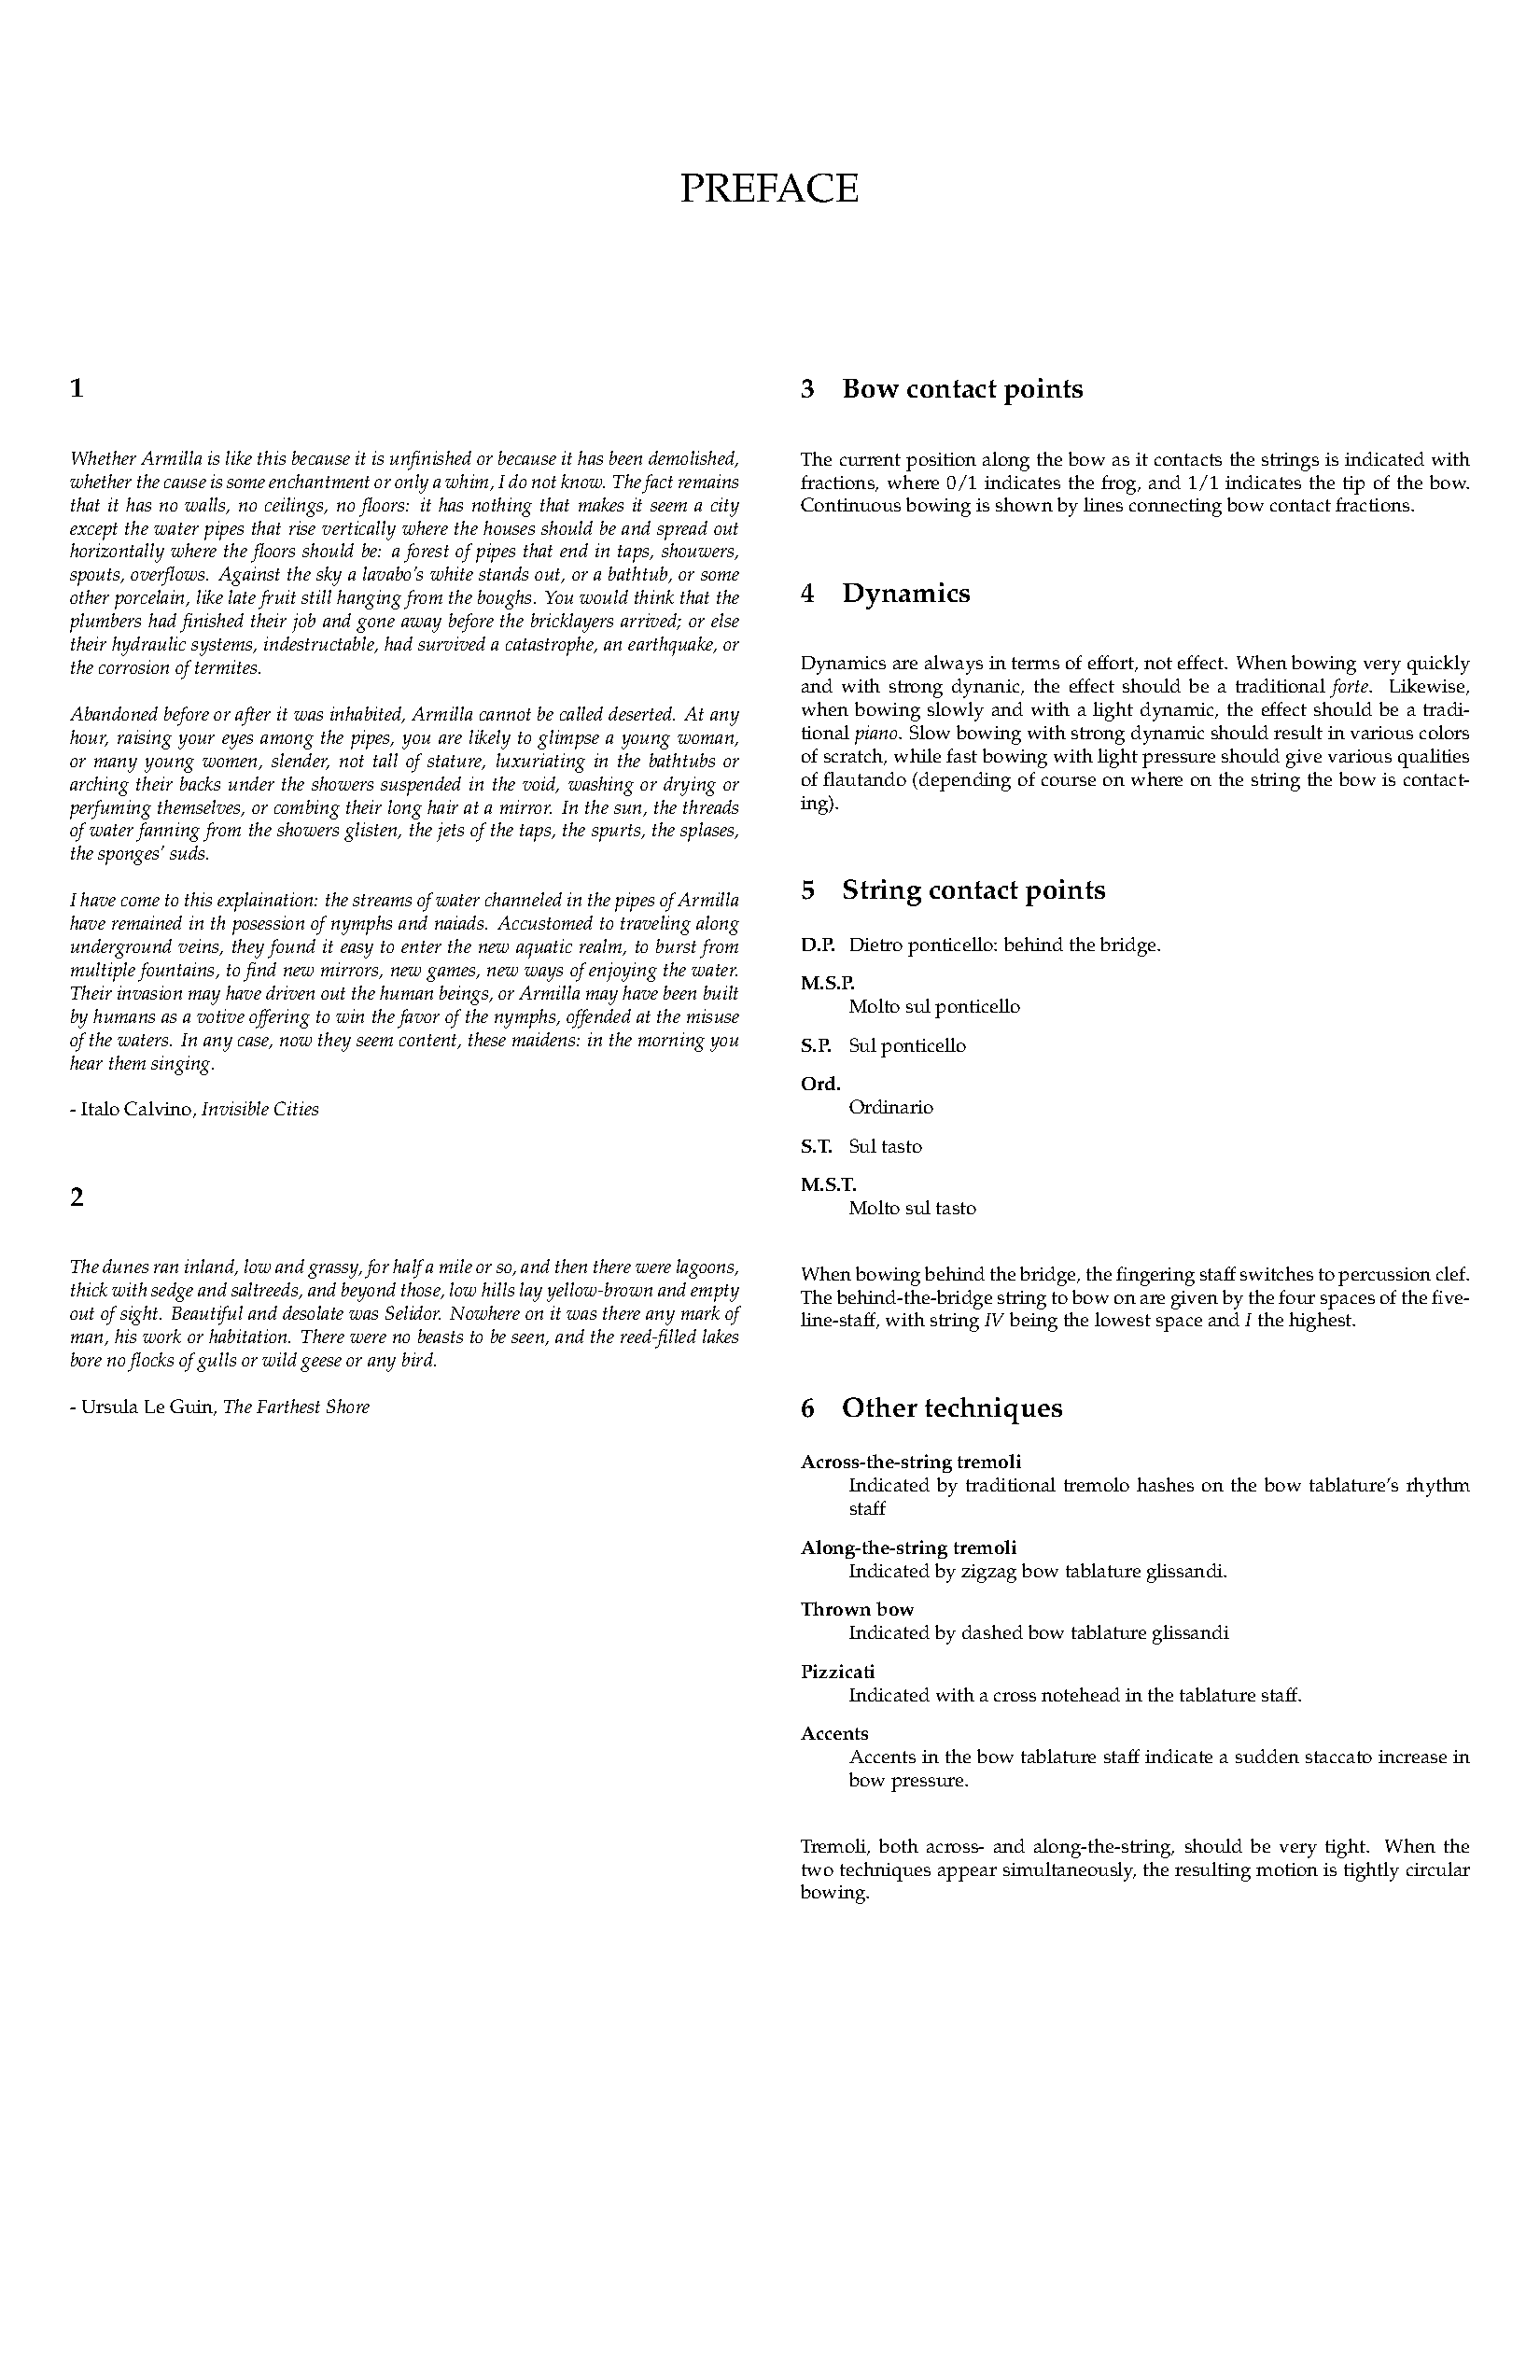
\includepdf[
    pages=-,
    pagecommand={\thispagestyle{plain}}
]{assets/dissertation-score-armilla.pdf}
%%%%%%%%%%%%%%%%%%%%%%%%%%%%%%%%%%%%%%%%%%%%%%%%%%%%%%%%%%%%%%%%%%%%%%%%%%%%%%%
%%%%%%%%%%%%%%%%%%%%%%%%%%%%%%%%%%%%%%%%%%%%%%%%%%%%%%%%%%%%%%%%%%%%%%%%%%%%%%%
\chapter{\emph{Invisible Cities (iii): Ersilia} (2015)}
%%%%%%%%%%%%%%%%%%%%%%%%%%%%%%%%%%%%%%%%%%%%%%%%%%%%%%%%%%%%%%%%%%%%%%%%%%%%%%%
%%%%%%%%%%%%%%%%%%%%%%%%%%%%%%%%%%%%%%%%%%%%%%%%%%%%%%%%%%%%%%%%%%%%%%%%%%%%%%%

\begin{singlespacing}
\begin{flushright}
A composition for chamber orchestra \\
\vspace*{\baselineskip}
Premi\`{e}red by Ensemble Dal Niente \\
on Saturday May 16th, 2015 \\
in Paine Hall, Harvard University
\end{flushright}
\end{singlespacing}

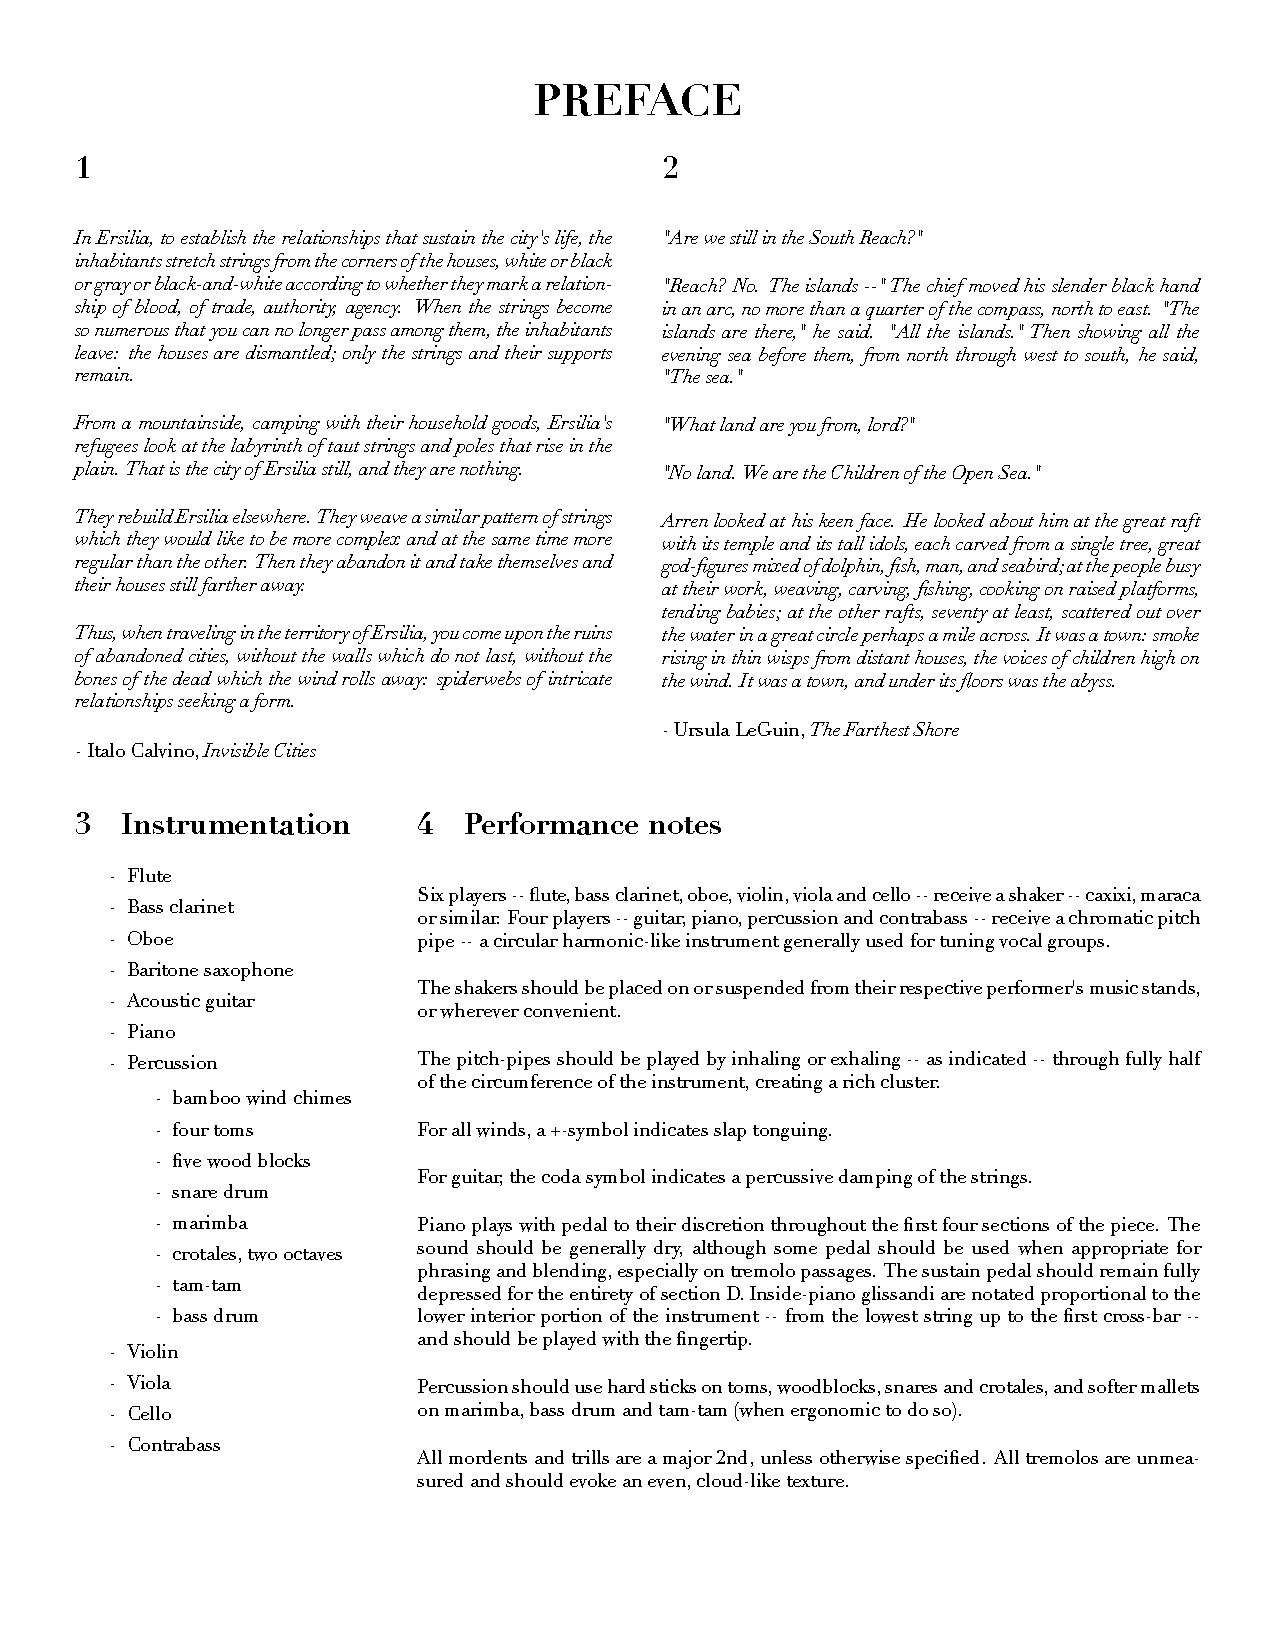
\includepdf[
    pages=-,
    pagecommand={\thispagestyle{plain}}
]{assets/dissertation-score-ersilia.pdf}


\begin{appendices}
    \input{appendices/consort/index.tex}
\input{appendices/zaira/index.tex}
\input{appendices/armilla/index.tex}
\end{appendices}

\singlespacing

% the back matter
\clearpage
\bibliography{references}
\addcontentsline{toc}{chapter}{References}
\bibliographystyle{apalike2}

\newpage

% If you do want an image in the colophon:
\begin{figure}
    \vspace{50pt}
    \centering
    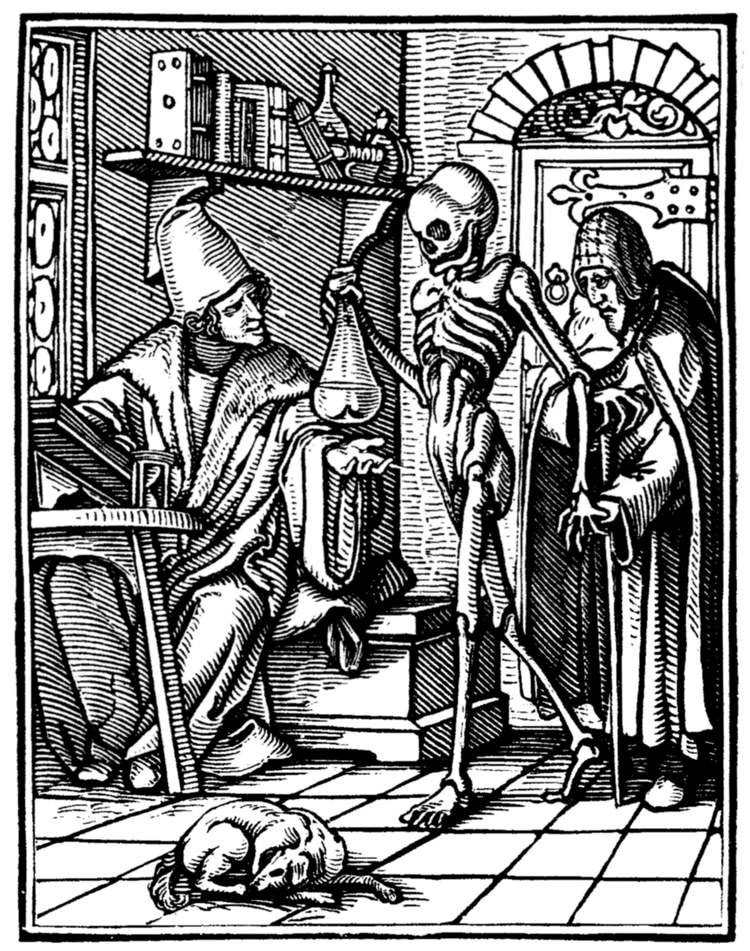
\includegraphics[width=0.51\textwidth]{endmatter/holbein-physician.jpg}
    \\
    \emph{The Physician}
    \\
    from Hans Holbein's \emph{Danse Macabre}
\end{figure}

% If you don't want an image in the colophon:
% \vspace*{200pt}

\begin{center}
\parbox{200pt}{\lettrine[lines=3,slope=-2pt,nindent=-4pt]{\textcolor{SchoolColor}{T}}{his
thesis was typeset} using \LaTeX, originally developed by Leslie Lamport and
based on Donald Knuth's \TeX. The body text is set in 11 point Egenolff-Berner
Garamond, a revival of Claude Garamont's humanist typeface. }
\end{center}

\end{document}